\documentclass{standalone}

\usepackage{amssymb}
\usepackage{tikz}
\usetikzlibrary{intersections}

\newcommand{\PP}{\mathbb P}

\begin{document}

    %\includegraphics[scale=.5]{monodromy.pdf}
    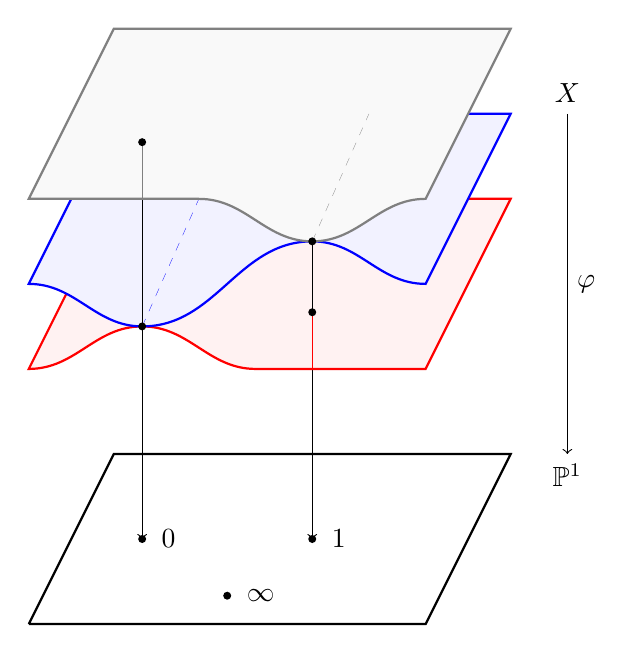
\begin{tikzpicture}[scale=.36]
      % sheet 1 fill
      \fill[red!5!white] (0,9) to[out=0,in=-180] (4,10.5) to[out=0,in=-180] (8,9) -- (14,9) -- (17,15) -- (3,15) -- cycle;
      % sheet 2 fill
      \fill[blue!5!white] (0,12) to[out=0,in=-180] (4,10.5) to[out=0,in=-180] (10,13.5) to[out=0,in=-180] (14,12) -- (17,18) -- (3,18) -- cycle;
      % sheet 3 fill
      \fill[gray!5!white] (0, 15) -- (6,15) to[out=0,in=-180] (10,13.5) to[out=0,in=-180] (14,15) -- (17,21) -- (3,21) -- cycle;
      % base
      \draw[thick] (0,0)--(14,0)--(17,6)--(3,6)--(0,0);
      % projection to 0
      \draw[<-, black, thin] (4,3) -- (4,15);
      \draw[gray, thin] (4,15) -- (4,17);
      % projection to 1
      \draw[<-, black, thin] (10,3) -- (10,9);
      \draw[red, thin] (10,9) -- (10,11);
      \draw[black, thin] (10,11) -- (10,13.5);
      % branching
      \draw[blue, ultra thin, dashed] (4,10.5)--(6,15);
      \draw[gray, ultra thin, dashed] (10,13.5)--(12,18);
      % sheet 1 outline
      % we can't intersect with the sheet 2 fill because the intersections library
      % can't handle parallel lines
      % https://tex.stackexchange.com/a/581465/6934
      \path[name path=seg-2] (0,12) to[out=0,in=-180] (4,10.5);
      \path[name path=seg-1] (3,15) -- (0,9);
      \draw[red, thick, name intersections={of=seg-2 and seg-1}] (intersection-1) -- (0,9) to[out=0,in=-180] (4,10.5) to[out=0,in=-180] (8,9) -- (14,9) -- (17,15) -- (15.5,15);
      % sheet 2 outline
      \draw[blue, thick] (1.5,15) -- (0,12) to[out=0,in=-180] (4,10.5) to[out=0,in=-180] (10,13.5) to[out=0,in=-180] (14,12) -- (17,18) -- (15.5,18);
      % sheet 3 outline
      \draw[gray, thick] (0, 15) -- (6,15) to[out=0,in=-180] (10,13.5) to[out=0,in=-180] (14,15) -- (17,21) -- (3,21) -- cycle;
      % points
      \fill [black] (4,3) circle (4pt);
      \node at (4,3) [label=right:$0$] {};
      \fill [black] (10,3) circle (4pt);
      \node at (10,3) [label=right:$1$] {};
      \fill [black] (10,11) circle (4pt);
      %\node at (12.5,11) {$x=1/2$};
      \fill [black] (4,10.5) circle (4pt);
      %\node at (6.5,10.5) {$x=0$};
      \fill [black] (4,17) circle (4pt);
      %\node at (7,17) {$x=-3/2$};
      \fill [black] (10,13.5) circle (4pt);
      %\node at (13,13.5) {$x=-1$};
      \fill [black] (7,1) circle (4pt);
      \node at (7,1) [label=right:$\infty$] {};
      % misc
      %\node[red] at (-1,9) {$1$};
      %\node[blue] at (-1,12) {$2$};
      %\node[gray] at (-1,15) {$3$};
      \node at (19,18.75) {$X$};
      \node at (19,5.25) {$\PP^1$};
      \draw[black,->] (19,18) to node[right]{$\varphi$} (19,6);
    %\node at (22,12) {z=\phi(x)=2x^3+3x^2$};
      %\node at (24,12) {$\phi(x)=2x^3+3x^2$};
    \end{tikzpicture}
\end{document}
